\documentclass[UTF8,a4paper,11pt,fontset=fandol]{ctexart}

\usepackage[a4paper,margin=2.2cm]{geometry}
\usepackage{hyperref}
\usepackage{graphicx}
\usepackage{booktabs}
\usepackage{longtable}
\usepackage{array}
\usepackage{ragged2e}
\usepackage{caption}
\usepackage{float}
\usepackage{xcolor}

\newcolumntype{L}[1]{>{\RaggedRight\arraybackslash}p{#1}}
\setlength{\tabcolsep}{4pt}
\setlength{\emergencystretch}{1.5em}
\setlength{\intextsep}{8pt}
\renewcommand{\arraystretch}{1.08}
\captionsetup{font=small,labelfont=bf,skip=5pt}
\setlength{\parskip}{0.3em}

\title{《可视化导论》课程网站重构}
\author{可视化导论第四次作业}
\date{2026年10月}

\hypersetup{colorlinks=true,linkcolor=blue,urlcolor=blue}
\pagestyle{plain}

\begin{document}

\maketitle

\section{作品概述}

原课程站以章节为单位组织（\url{https://cinger007.github.io/vis/}），每章是一套独立的 HTML、CSS 和 JavaScript，页面中包含讲解、关键代码和演示三个 Tab。这种结构便于单独维护某一章，但公共导航、语言切换和演示逻辑在页面之间重复，阅读时也要在多个页面之间跳转。

本次作业在保留原有教学内容的前提下做了整体重构：页面与组件改用 Vue 3 + TypeScript + Vite，课程内容改为 Markdown 与配置驱动，演示改为按需加载的独立模块，并补上站内搜索、全屏、图表导出和移动端布局。五章 27 个小节、第一章 5 个独立演示、14 个现存补充案例和 10 份中英讲义全部保留。

课程站入口：\url{https://vis.starlab.top/hw04/}。源码：\url{https://github.com/InvalidNamee/cinger-vis-rebuild}，fork 自 \texttt{cinger007/vis}。站点仍是纯静态前端，没有后端，也没有加入视频或大体积媒体；构建产物约 10\,MB，保持纯静态部署。

下面分两部分说明：第二节是读者能直接看到的变化，第三节是不太容易看到、但决定维护方式和加载行为的架构调整。两节都用“改之前 / 改之后 / 作用”对照。

\section{界面与交互改进}

表~\ref{tab:visible} 按页面和交互顺序列出九处可见变化。

{\footnotesize
\begin{longtable}{@{}L{1.8cm}L{4.4cm}L{4.7cm}L{3.7cm}@{}}
\caption{可见修改：改之前、改之后与作用}\label{tab:visible}\\
\toprule
变化点 & 改之前 & 改之后 & 作用 \\
\midrule
\endfirsthead
\toprule
变化点 & 改之前 & 改之后 & 作用 \\
\midrule
\endhead
\bottomrule
\endfoot
视觉与图标 & 靛蓝渐变、白卡片、各页独立样式，功能图标用 emoji。 & 以蓝色和珊瑚色为主，统一页面配色，1160\,px 居中布局，Lucide SVG 图标，磨砂吸顶导航。 & 风格统一，层级清楚，不再靠 emoji 区分功能。 \\
顶部导航 & 章节页各自一套深色 header 和链接行，首页用页内锚点；窄屏拥挤。 & 全站吸顶胶囊导航：五章直达、补充案例、关于、搜索、GitHub、语言；当前项滑动高亮；$\le 1160$\,px 下拉，$\le 720$\,px 语言入菜单。 & 任何页面都能直接跳章，窄屏不挤，当前位置明确。 \\
首页 & 首屏、五章卡片、使用方式、关于全挤在一页；卡片带“已上线”徽标和 emoji。 & 首屏加五章卡片，每卡顶部一组数据母题插画（表格、流程、色板、散点、时序）；使用方式和关于独立成页。 & 首页专注课程目录，五章有图形索引，学习入口不被说明文字淹没。 \\
章节页与目录 & 220\,px 侧栏、1400\,px 内容、14\,px 正文；目录只在点击时高亮，点目录会强制切到演示 Tab。 & 页面最大宽度 1160\,px，侧栏 240\,px，正文 16\,px；代码高亮可复制；目录随滚动自动高亮；点目录只定位、不改 Tab；手机目录可收起。 & 长章阅读知道位置；点目录不打断阅读；手机也能用目录。 \\
三 Tab 与 URL & 原生按钮加 \texttt{display:none}；Tab 状态不写 URL，分享或刷新只回到章节，并落到演示 Tab。 & Reka UI Tabs，键盘可操作；每节用 \texttt{tab-} 加小节 ID 记住 Tab；语言、hash、Tab 可同时保留。 & 可精确分享“某章某节某 Tab”；刷新和前进后退不丢状态。 \\
站内搜索 & 没有搜索，只能翻目录或用浏览器查找。 & 顶栏搜索加 Command+K / Ctrl+K；覆盖正文、代码、演示、补充案例、关于；中英文索引、加权排序、高亮；结果定位到小节或 Tab，代码结果展开源码区。 & 查概念、函数、案例从“逐章翻”变成“一次输入”。 \\
全屏与导出 & 都没有；课堂投影只能缩小浏览器，图表只能截图。 & H2 小节全屏（含三 Tab），独立演示和补充案例的演示区可全屏，原生失败降级站内；登记 SVG 可导出 SVG 或白底高清 PNG，多图可选。 & 课堂投影更清楚；图表能进笔记、报告和课件。 \\
补充案例与关于 & 索引标题是文件名，案例页样式各异；“关于、使用方式”在首页，还写着“零依赖、无需 npm”。 & 标题改为可读描述，文件名降为辅助；按五章分组、待排期标记、材料下载；关于独立成页并按 Vue、npm、静态服务重写。 & 先知道案例讲什么再决定进；使用说明与实际运行方式一致。 \\
动效与可达性 & 只有 Tab 面板 200\,ms 淡入和卡片 hover 位移；没有减少动画处理。 & 卡片渐入、悬停缩放、母题绘制动画、导航当前项滑动；\texttt{prefers-reduced-motion} 下关闭动画；键盘焦点可见。 & 动效提示层级和位置，不是纯装饰；对减少动画用户友好。 \\
\end{longtable}
}

\section{架构方面的修改}

架构改动不像界面那样一眼可见，但决定了页面之间是否一致、演示加载是否拖慢首屏等。表~\ref{tab:arch} 按四个层面概括。

{\footnotesize
\begin{longtable}{@{}L{1.8cm}L{4.4cm}L{4.7cm}L{3.7cm}@{}}
\caption{架构修改：改之前、改之后与作用}\label{tab:arch}\\
\toprule
层面 & 改之前 & 改之后 & 作用 \\
\midrule
\endfirsthead
\toprule
层面 & 改之前 & 改之后 & 作用 \\
\midrule
\endhead
\bottomrule
\endfoot
页面与代码组织 & 每章、每个补充案例都是独立 HTML，各带自己的样式和脚本；公共导航和语言逻辑在页面间重复。 & Vue 3 + TypeScript + Vite 单页应用，路由组织首页、章节、演示、补充案例、关于；导航、页脚、语言、加载状态做成公共组件。 & 公共部分只维护一份；页面行为一致；新增章节或改样式不用逐页复制。 \\
内容与演示组织 & 正文、代码、提示框直接写在 HTML 里，中英文各一套标签；演示注册在全局对象，脚本从 CDN 加载。 & 课程内容拆成 Markdown，章节结构用配置描述；演示拆成独立模块，依赖通过 npm 打包。 & 改教学内容不动页面结构；演示互不干扰；核心演示不再依赖 CDN。 \\
加载与运行 & 打开一章就把该章所有演示渲染一遍；跳章靠整页刷新，演示状态直接丢失。 & 演示按需加载，首次切到演示 Tab 才加载对应模块；单页内切章不刷新，离开页面时取消请求、清理监听和动画。 & 首屏更轻；切章不残留；同一小节内切换 Tab 或语言时，演示状态保留。 \\
构建、部署与检查 & 改完直接上传静态文件；没有自动检查，内容和链接靠人工点。 & 构建生成带哈希的静态产物，统一处理子目录基路径，hash 路由不需要 SPA 回退；旧入口有跳转；提供内容校验、单元测试和浏览器验收脚本。 & 部署到 \texttt{/hw04/} 子路径不会 404；迁移不丢内容、旧链接不断；改动后可快速回归。 \\
\end{longtable}
}

\clearpage
\section{页面截图}

\begin{figure}[H]
  \centering
  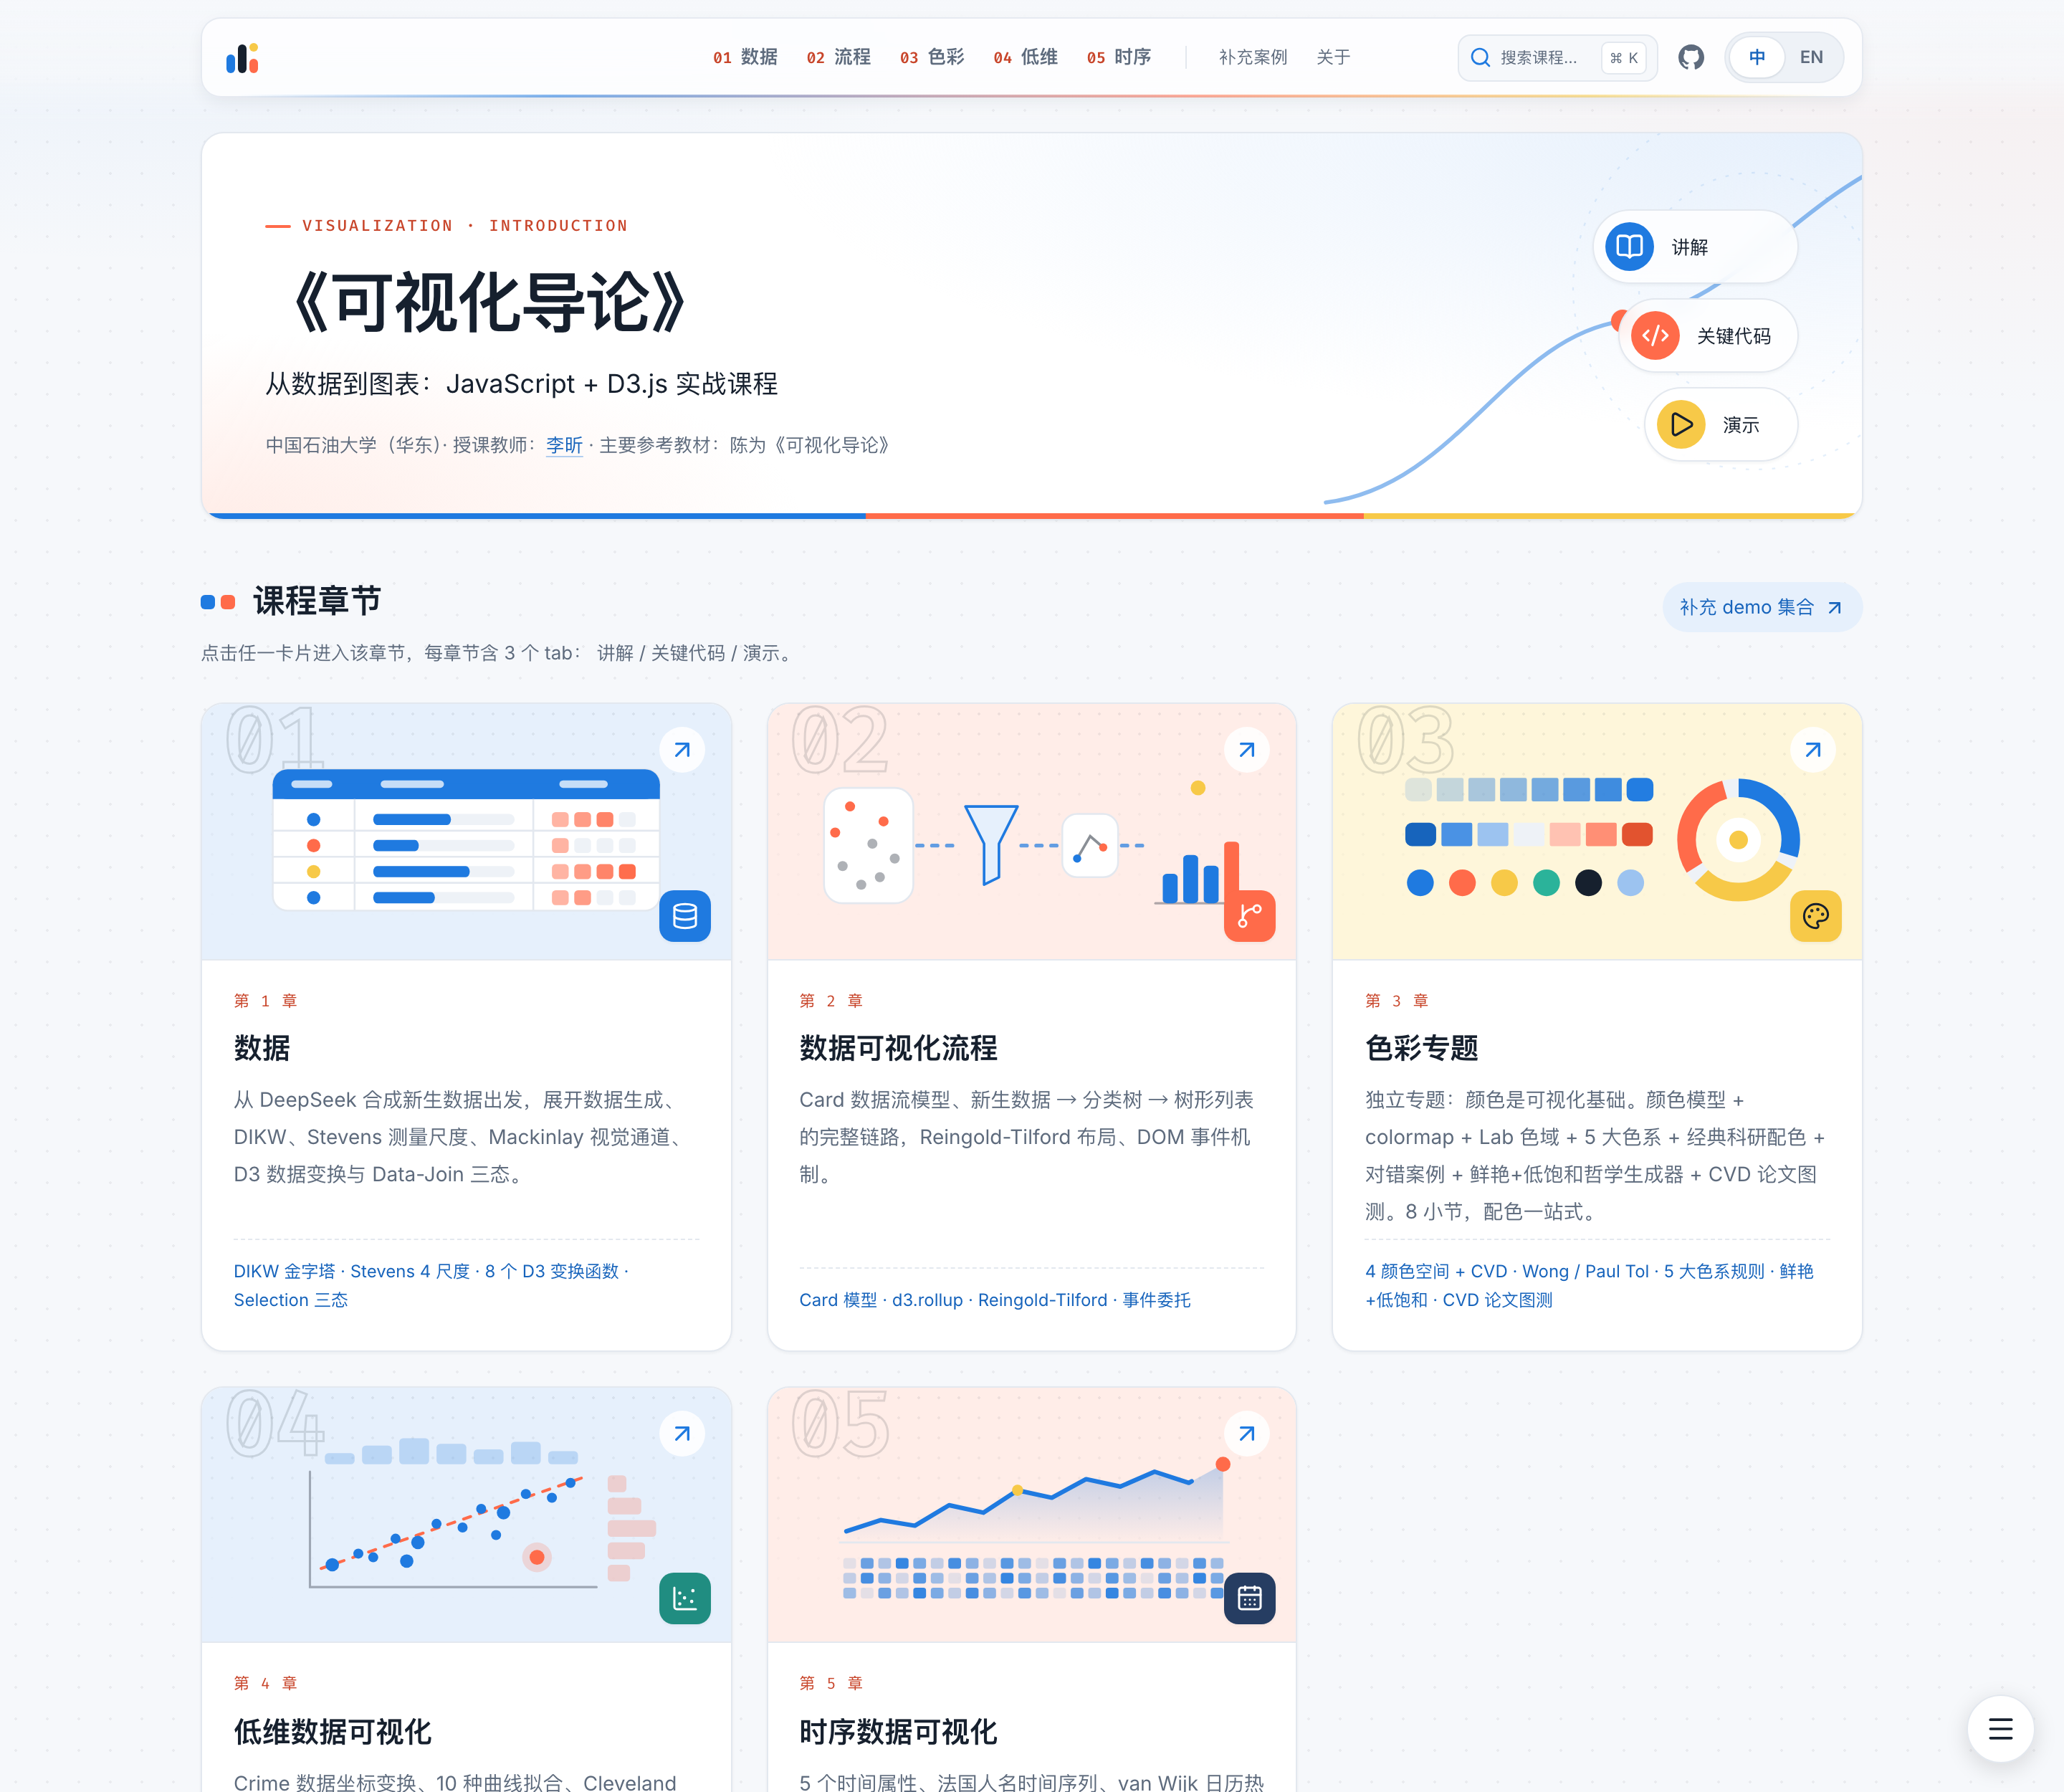
\includegraphics[width=0.7\textwidth]{images/home.png}
  \caption{重构后的首页。顶部是五章直达导航、搜索和语言切换；首屏说明课程定位，下面五张章节卡片各配一组数据母题插画。}
  \label{fig:home}
\end{figure}

\begin{figure}[H]
  \centering
  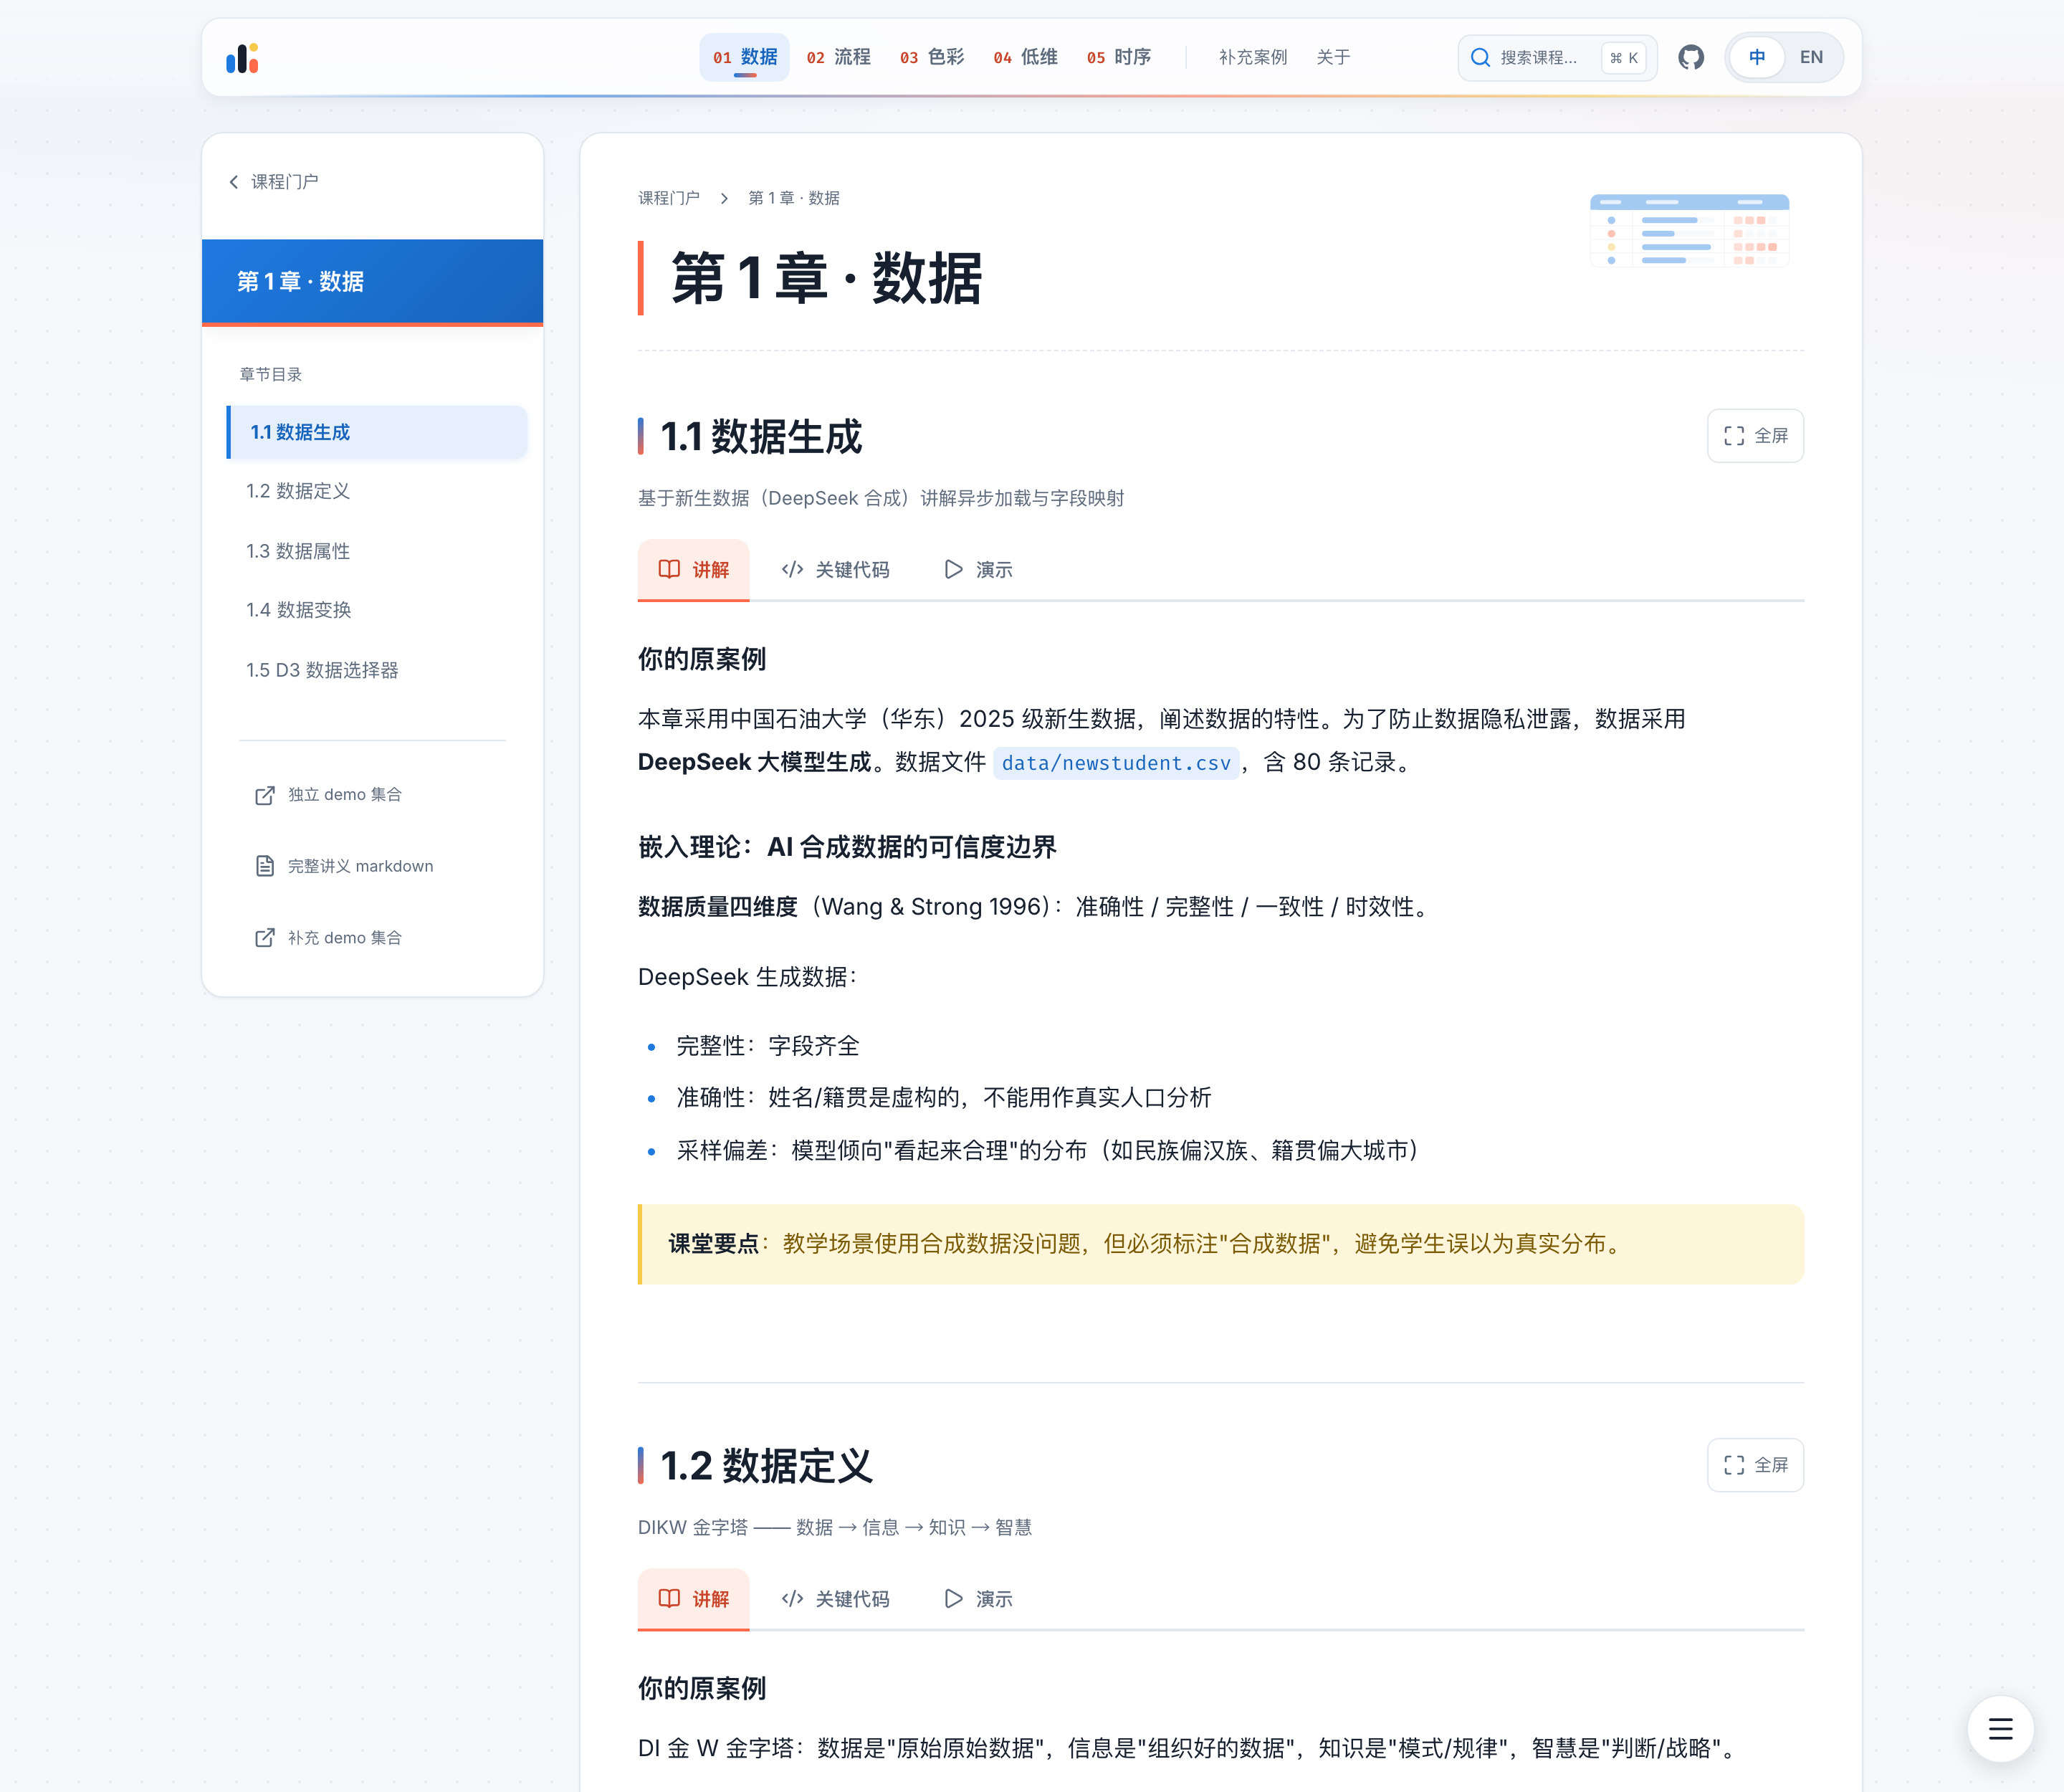
\includegraphics[width=0.7\textwidth]{images/lesson.png}
  \caption{章节页。左侧目录随滚动高亮当前小节；每个小节保留讲解、关键代码、演示三个 Tab，标题右侧可全屏。}
  \label{fig:lesson}
\end{figure}

\begin{figure}[H]
  \centering
  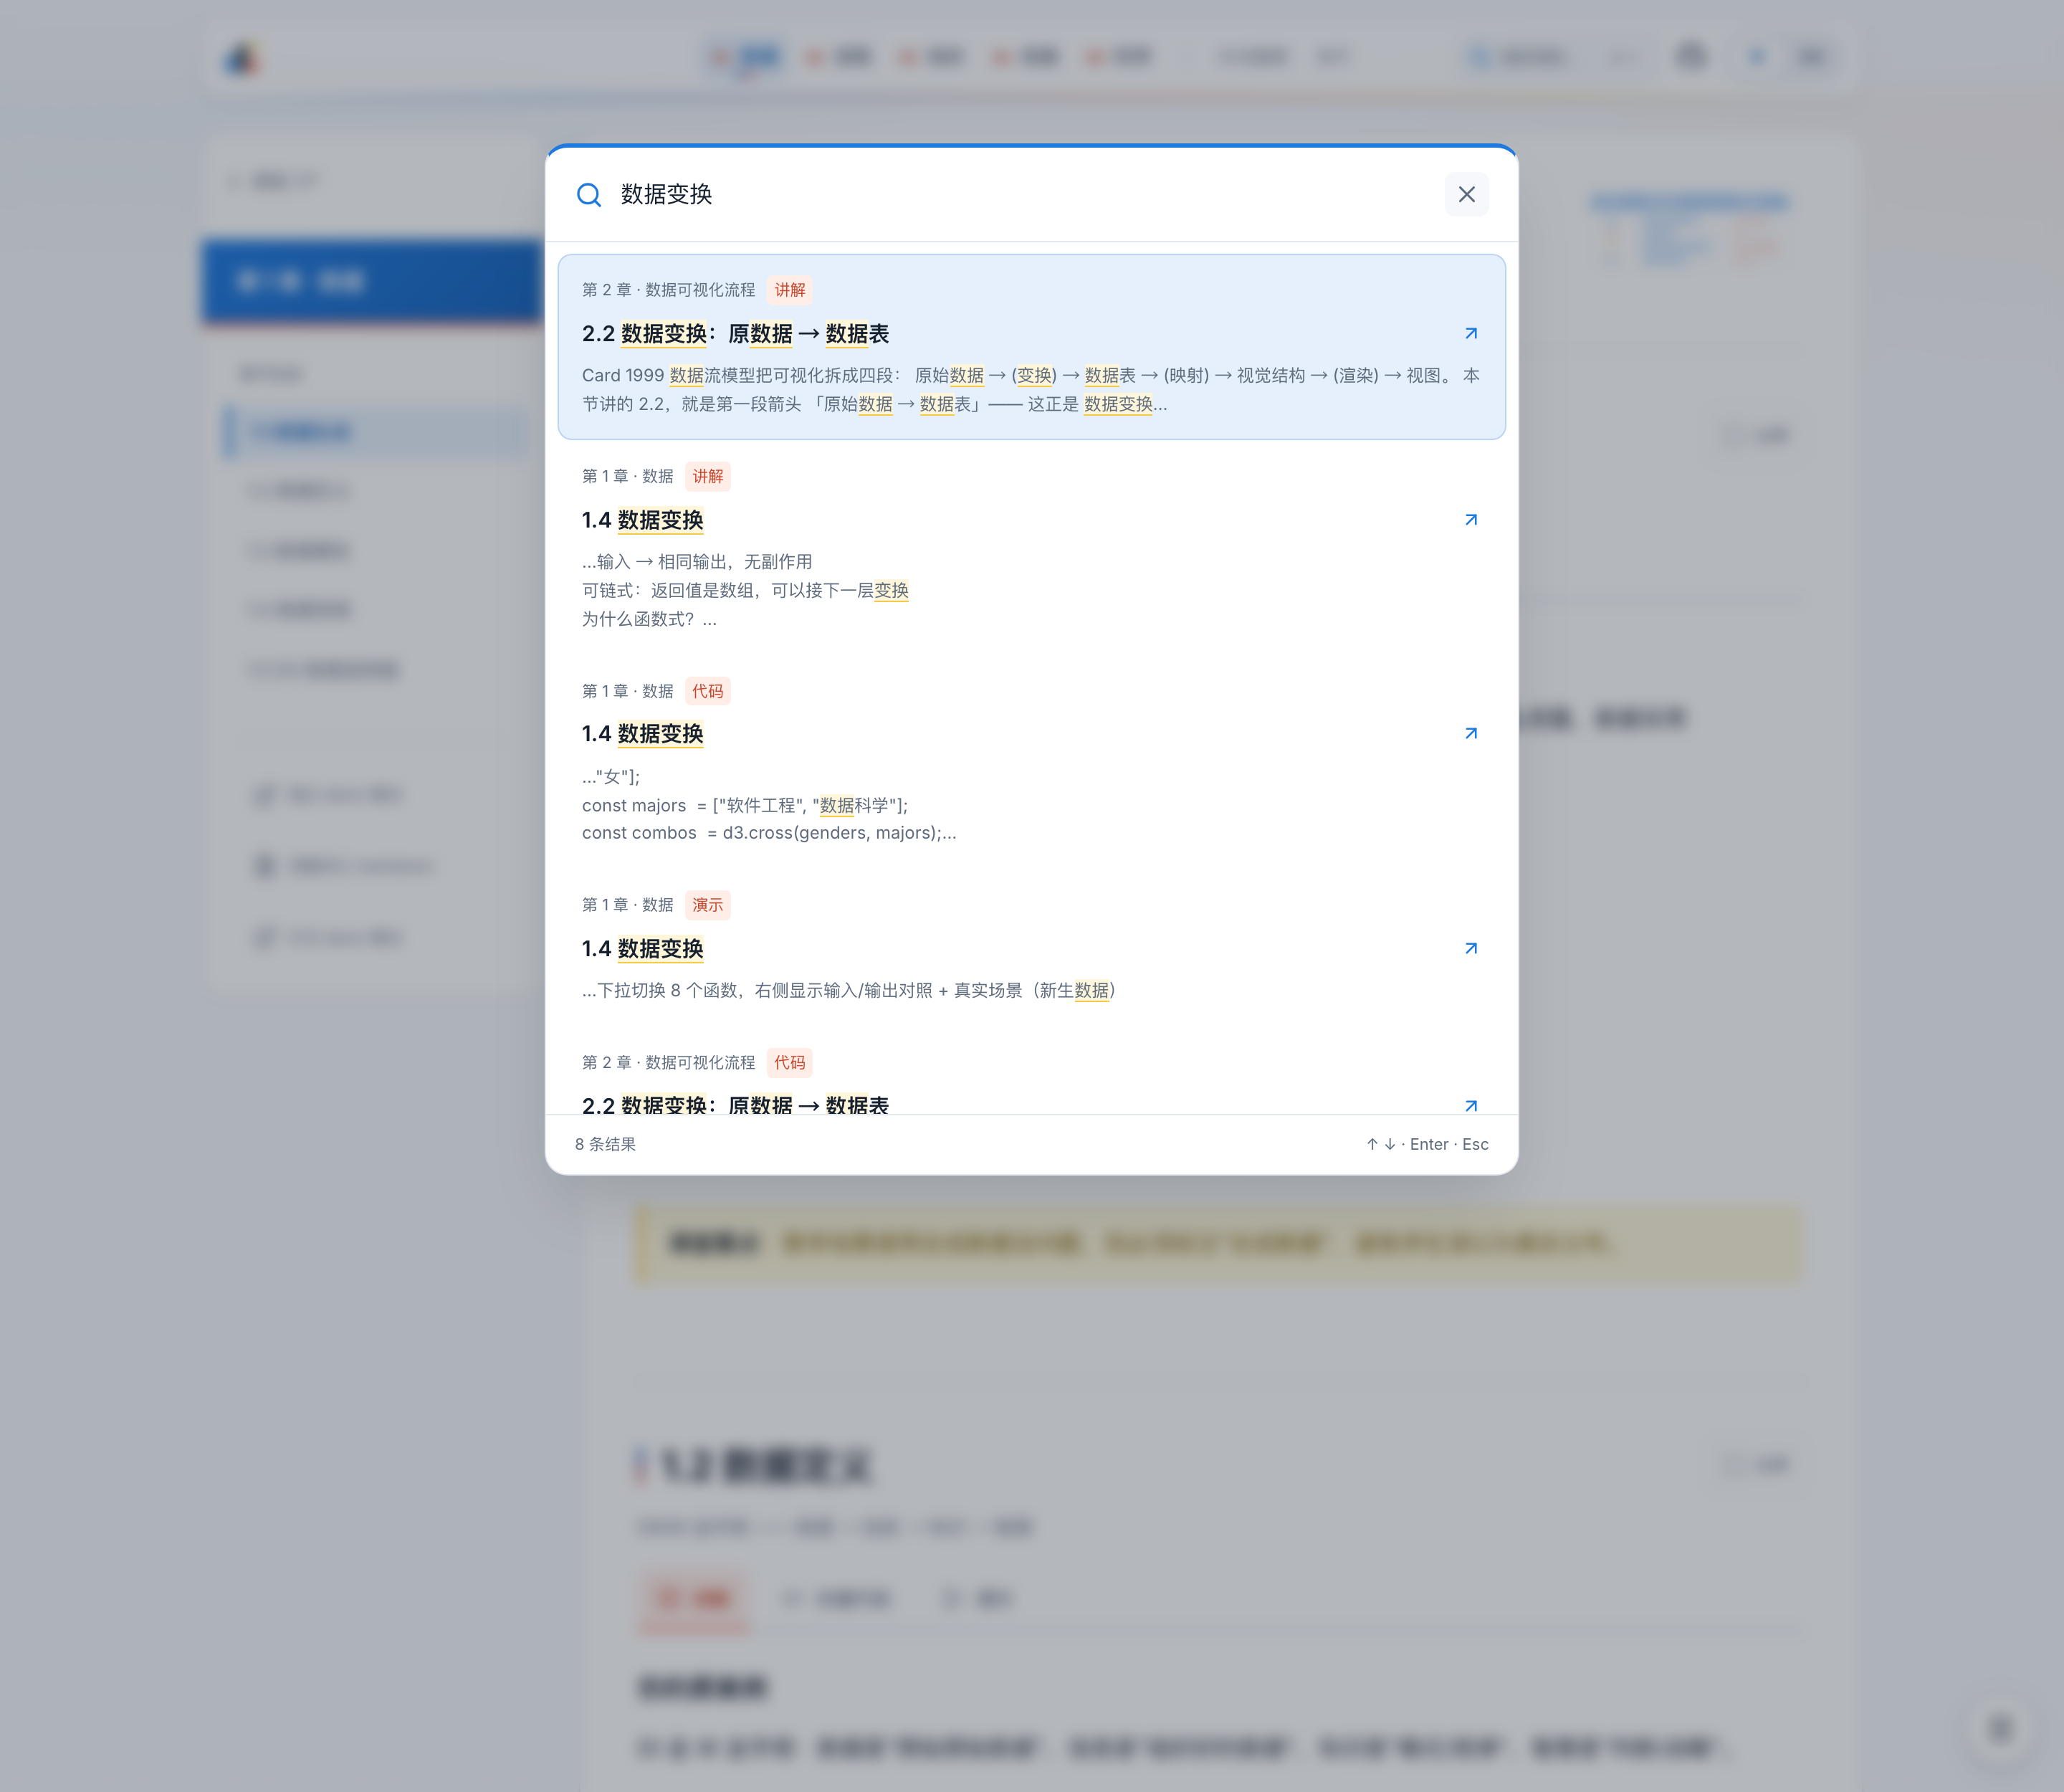
\includegraphics[width=0.64\textwidth]{images/search.png}
  \caption{站内搜索。输入“数据变换”后同时命中正文、代码和演示，命中词高亮；结果可直接跳到对应小节和 Tab。}
  \label{fig:search}
\end{figure}

\begin{figure}[H]
  \centering
  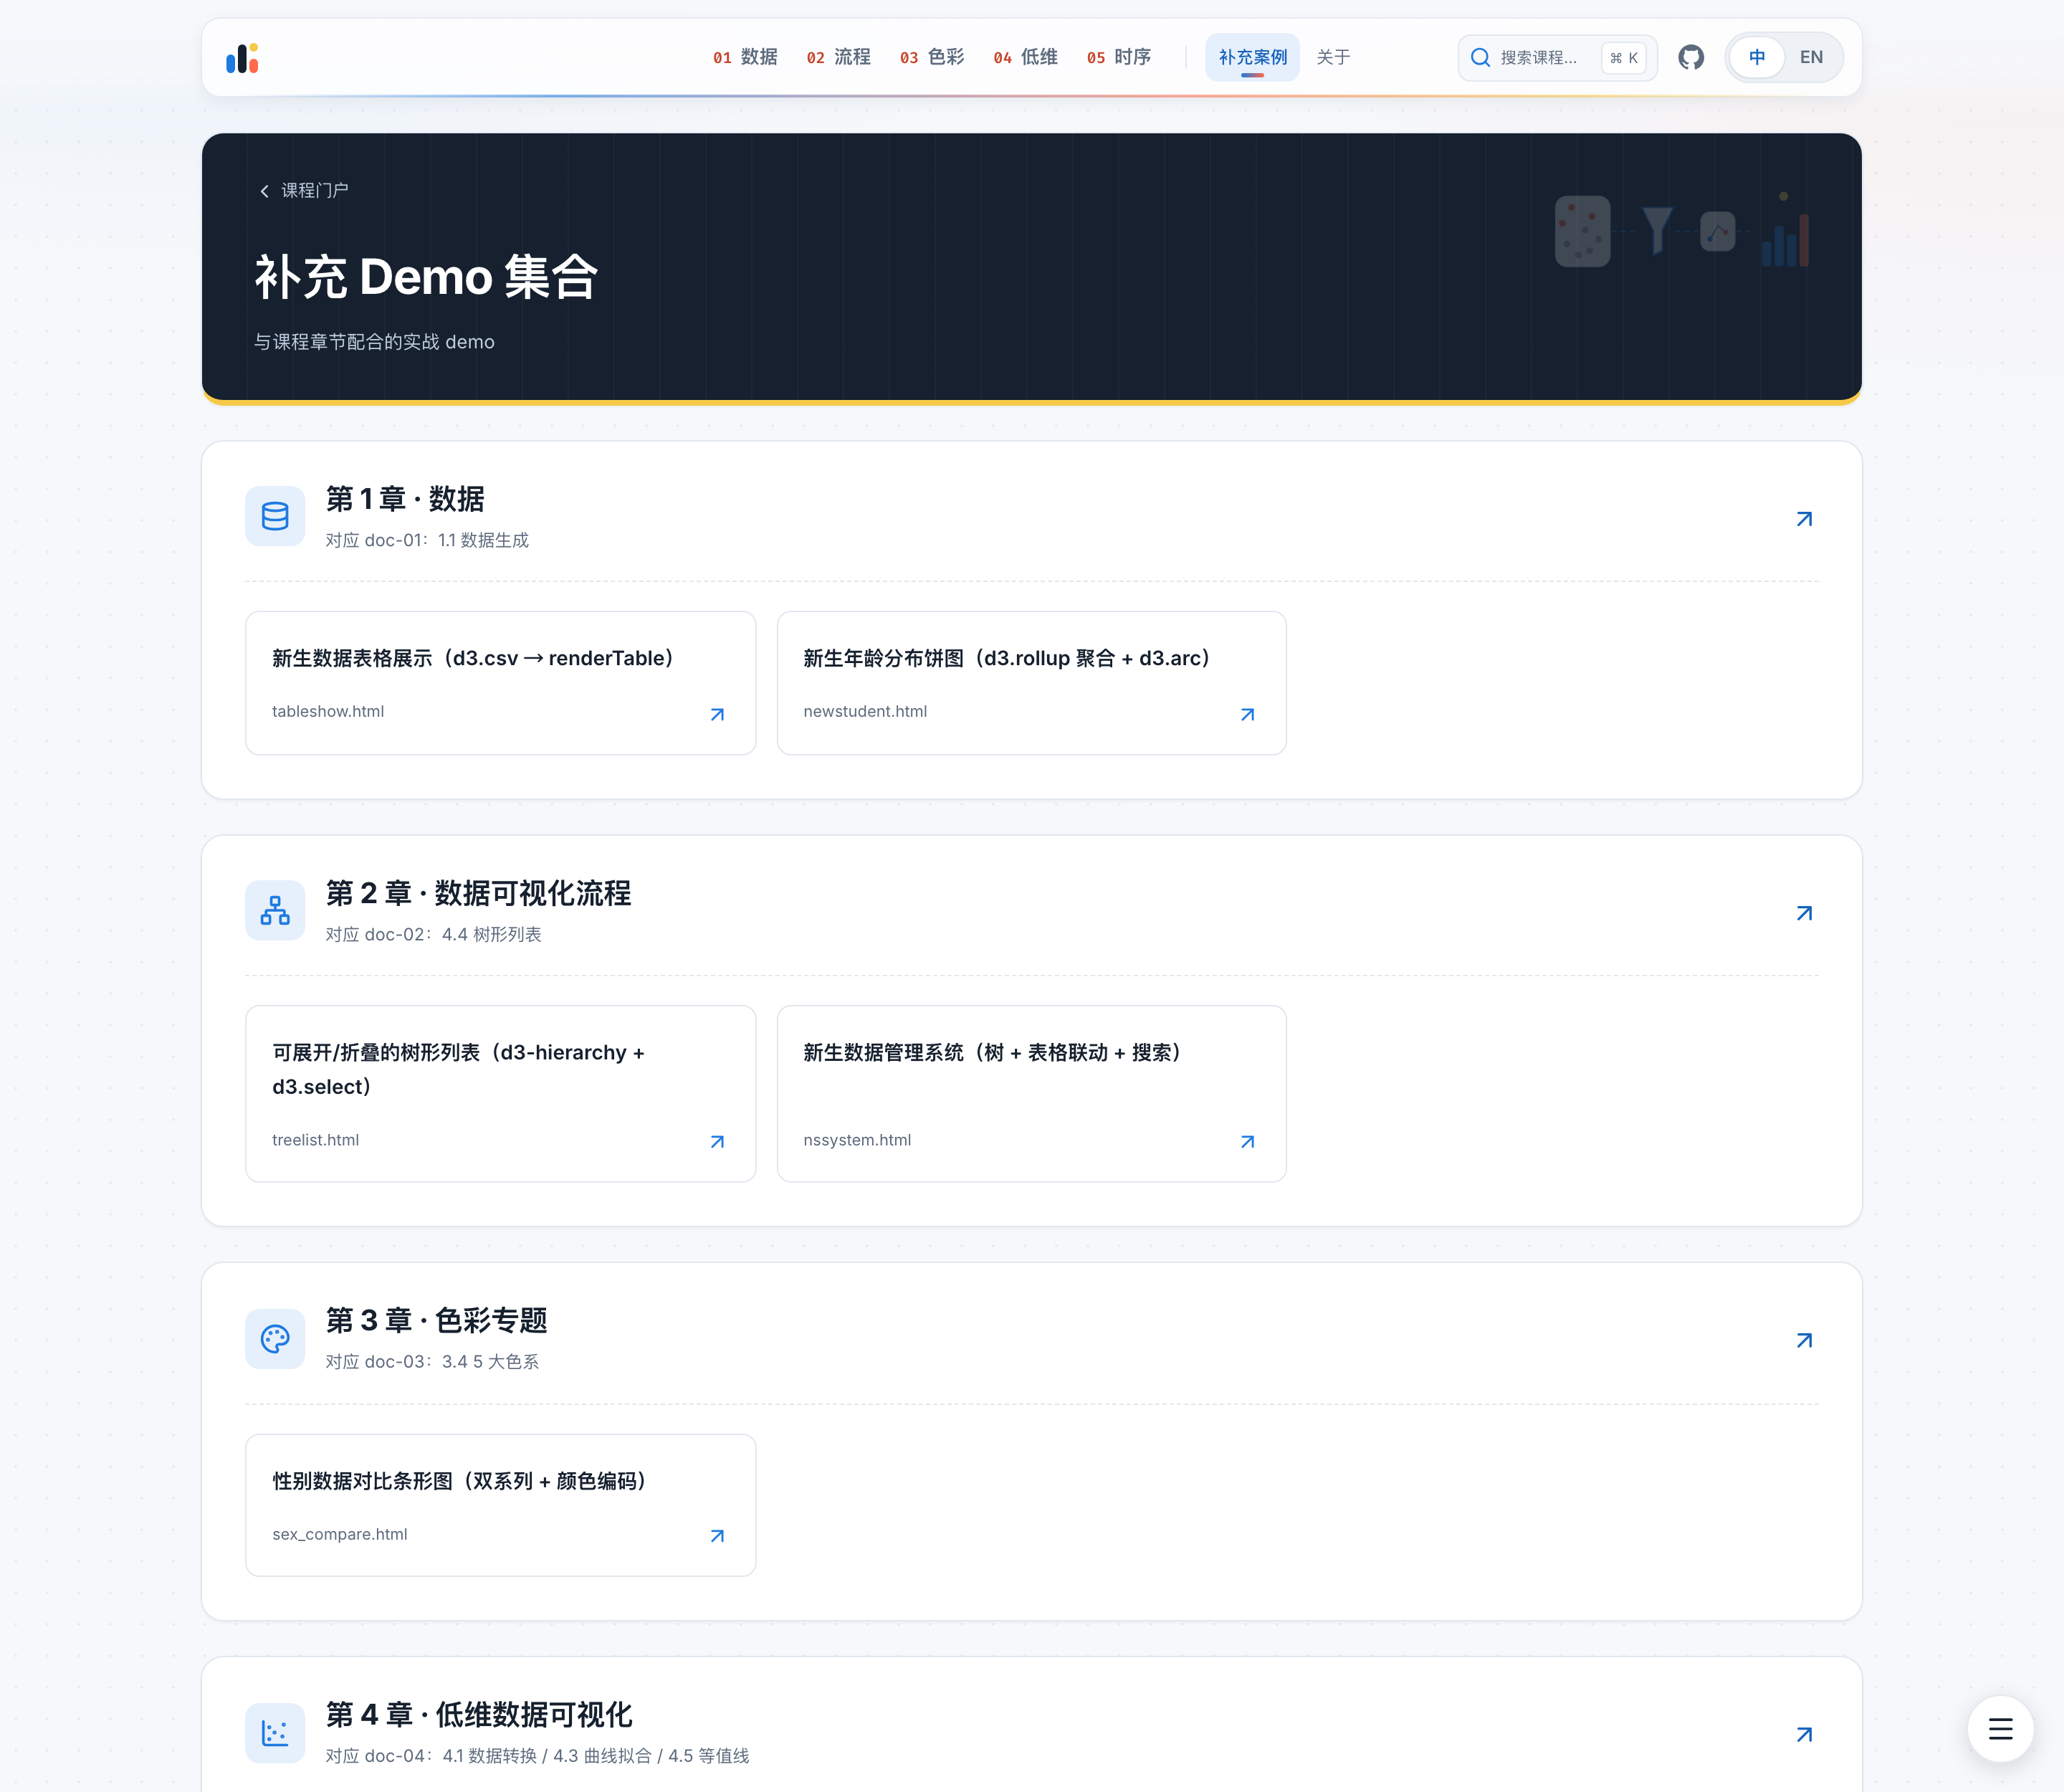
\includegraphics[width=0.56\textwidth]{images/supplementary.png}\hspace{0.02\textwidth}%
  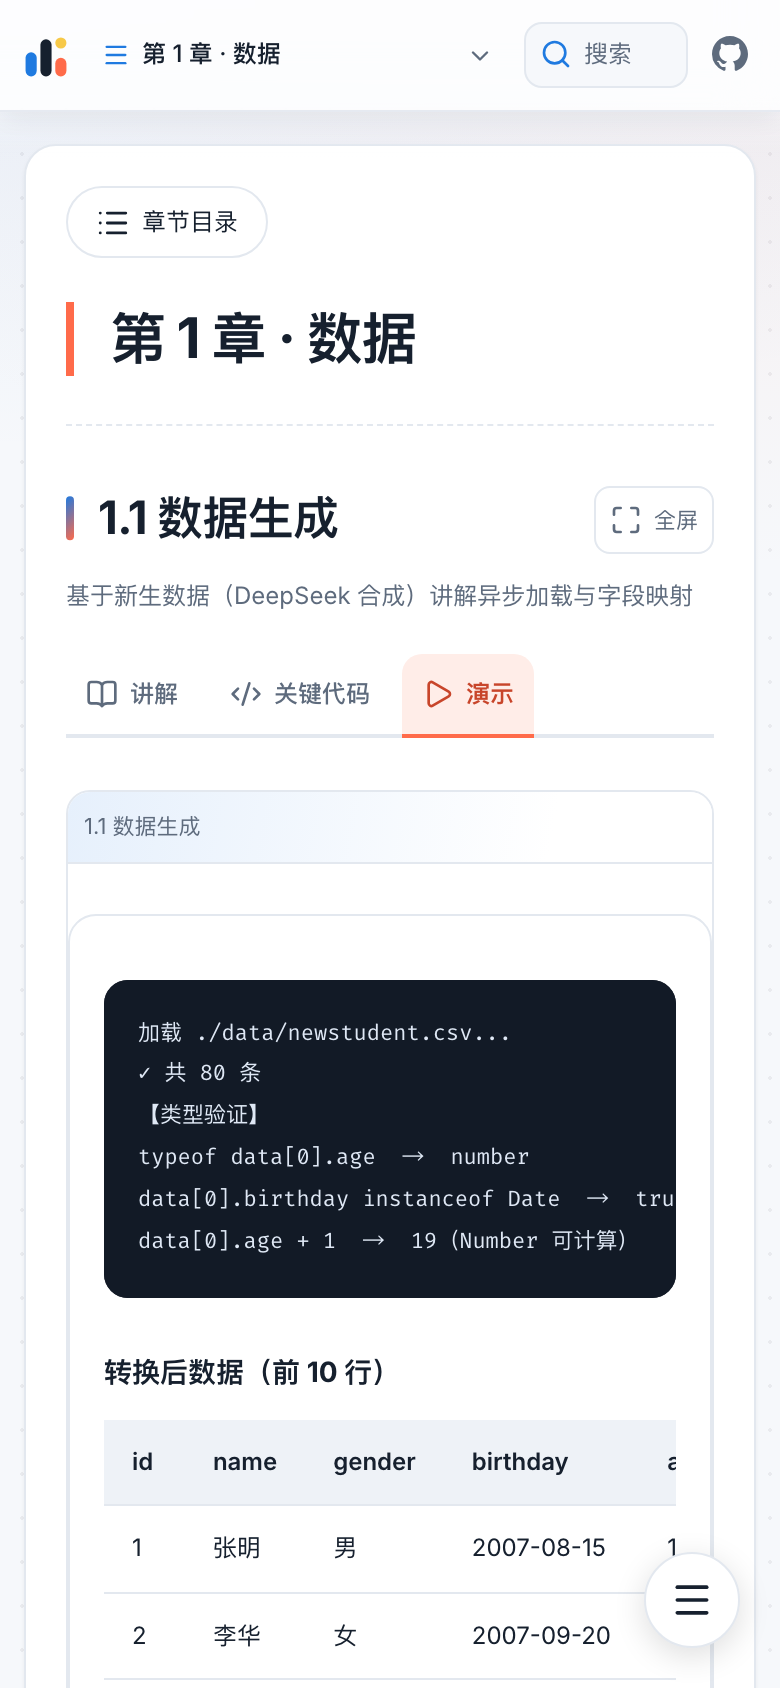
\includegraphics[height=6.2cm]{images/mobile.png}
  \caption{左：补充案例索引按五章分组，标题改为可读描述，文件名作为辅助信息。右：390\,px 手机端，导航收成下拉菜单，目录可展开，演示区局部滚动。}
  \label{fig:supp}
\end{figure}

\end{document}
